\section{量子力学导论}
\subsection{德布罗(de Broglie)意波}
\begin{itemize}
\item \textbf{推导}: 由假设$E=h\nu$得
\[
E=h\nu=h\frac{1}{\tau^*}=h\frac{v}{v\tau^*}=h\frac{v}{\lambda} \ \
\footnote{偷换概念: $v\tau^*=\lambda$ ,其中$v$是粒子运动速度}
\]
又由爱因斯坦质能方程(亦属假设, 未证实): $E=mc^2$将光速$c$偷换为$v$得
\[
E=mv^2
\]
由以上两式联立可得
\[
\lambda=\frac{h}{mv}
\]
\item \textbf{结论}: 可见推导是有问题, 推导的前提依据都是假说, 并且推导本身就有问题. 
\end{itemize}
\subsection{波与粒子的区别}
粒子携带质量, 符合动力学公式;波不携带质量(目前没有证据表明波携带质量),符合波的传播公式.请\textbf{思考}: 
\begin{itemize}
\item 定量描述波与粒子的区别?
\item 波干涉中的确定因素与电子衍射实验中的不确定因素, 电子衍射实验能否证明电子具有波动性?
\end{itemize}

\subsection{戴维孙(Davisson)-革末(Germer)实验}
戴维孙-革末实验用盖革记数器控测各个方向, 发现了有强弱分布. 戴维孙-革末实验能否说电子具有波动性. 
\begin{figure}[!htb]
\centering
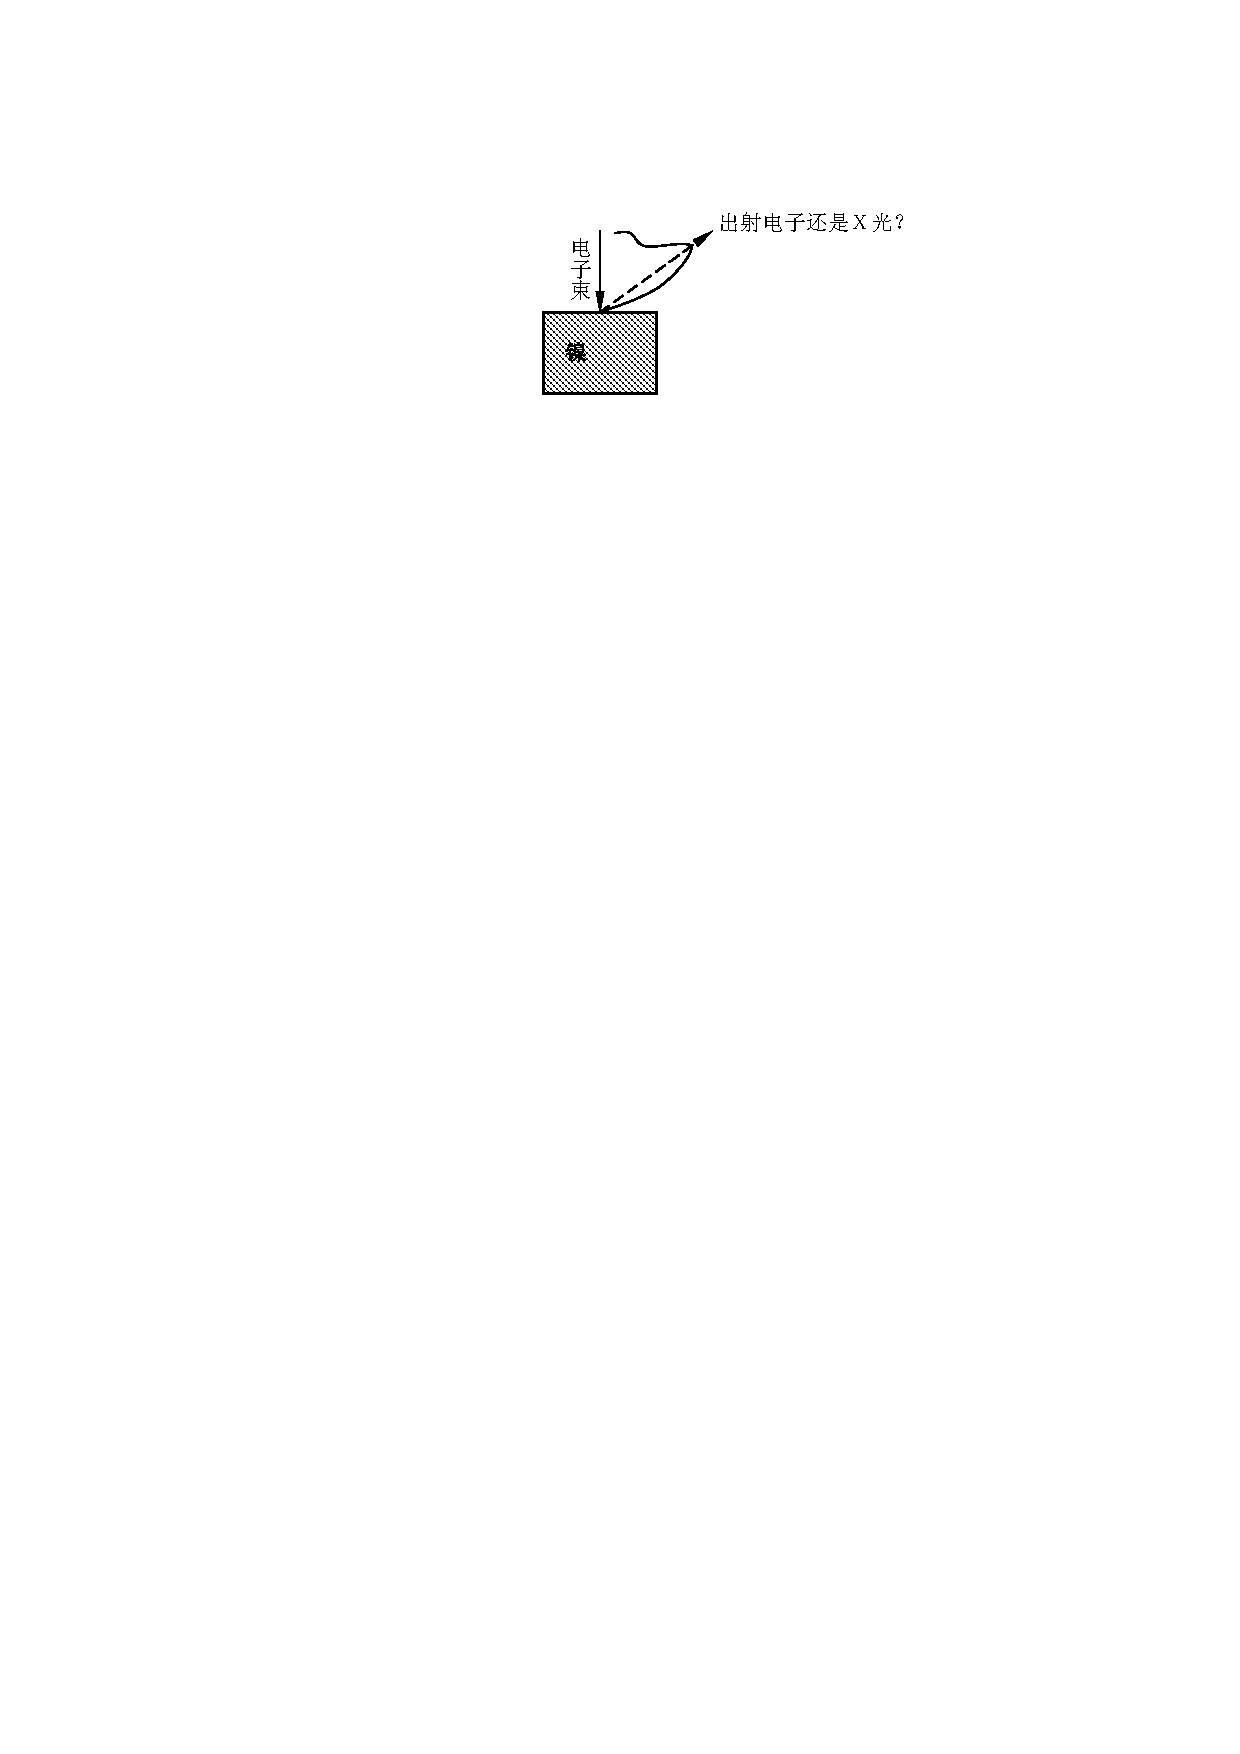
\includegraphics[width=0.4\textwidth]{fig16.pdf}
\caption{戴维孙-革末实验}
\end{figure}
事实上存在很大问题: 不能排除高能电子轰击材料而向各个方向上产生的x射线; 另外对于高能电子的轰击, 轰击后的速度几乎不可能与轰击前相同. 
